\documentclass[a4paper,11pt]{exam}
%\printanswers % pour imprimer les réponses (corrigé)
\noprintanswers % Pour ne pas imprimer les réponses (énoncé)
\addpoints % Pour compter les points
% \noaddpoints % pour ne pas compter les points
%\qformat{\textbf{\thequestion ) } }
%\qformat{\textbf{\thequestion )}} % Pour définir le style des questions (facultatif)
\usepackage{color} % définit une nouvelle couleur
\shadedsolutions % définit le style des réponses
% \framedsolutions % définit le style des réponses
\definecolor{SolutionColor}{rgb}{0.8,0.9,1} % bleu ciel
\renewcommand{\solutiontitle}{\noindent\textbf{Solution:}\par\noindent} % Définit le titre des solutions




\makeatletter

\def\maketitle{{\centering%
	\par{\huge\textbf{\@title}}%
	\par{\@date}%
	\par}}


\renewcommand{\thesubsection}{\Alph{subsection}.}   

\makeatother

\lhead{NOM Pr\'enom :}
\rhead{\textbf{Les r\'eponses doivent \^etre justifi\'ees et r\'edig\'ees}}
\cfoot{\thepage / \pageref{LastPage}}


%\usepackage{../../pas-math}
%\usepackage{../../moncours}


%\usepackage{pas-cours}
%-------------------------------------------------------------------------------
%          -Packages nécessaires pour écrire en Français et en UTF8-
%-------------------------------------------------------------------------------
\usepackage[utf8]{inputenc}
\usepackage[frenchb]{babel}
%\usepackage{numprint}
\usepackage[T1]{fontenc}
%\usepackage{lmodern}
\usepackage{textcomp}
\usepackage[french, boxed]{algorithm2e}
\usepackage{hyperref}


%-------------------------------------------------------------------------------

%-------------------------------------------------------------------------------
%                          -Outils de mise en forme-
%-------------------------------------------------------------------------------
\usepackage{hyperref}
\hypersetup{pdfstartview=XYZ}
%\usepackage{enumerate}
\usepackage{graphicx}
\usepackage{multicol}
\usepackage{tabularx}
\usepackage{multirow}
\usepackage{color}
\usepackage{eurosym}


\usepackage{anysize} %%pour pouvoir mettre les marges qu'on veut
%\marginsize{2.5cm}{2.5cm}{2.5cm}{2.5cm}

\usepackage{indentfirst} %%pour que les premier paragraphes soient aussi indentés
\usepackage{verbatim}
\usepackage{enumitem}
\usepackage{booktabs}
\usepackage[usenames,dvipsnames,svgnames,table]{xcolor}

\usepackage{variations}

%-------------------------------------------------------------------------------


%-------------------------------------------------------------------------------
%                  -Nécessaires pour écrire des mathématiques-
%-------------------------------------------------------------------------------
\usepackage{amsfonts}
\usepackage{amssymb}
\usepackage{amsmath}
\usepackage{amsthm}
\usepackage{tikz}
\usepackage{xlop}
\usepackage[output-decimal-marker={,}]{siunitx}
%-------------------------------------------------------------------------------

%-------------------------------------------------------------------------------
%                  -Nécessaires pour écrire des formules chimiquess-
%-------------------------------------------------------------------------------

\usepackage[version=4]{mhchem}

%-------------------------------------------------------------------------------
% Pour pouvoir exploiter les fichiers directement dans beamer
\newcommand{\pause}{\ }
%-------------------------------------------------------------------------------
%                    - Mise en forme avancée
%-------------------------------------------------------------------------------

\usepackage{ifthen}
\usepackage{ifmtarg}


\newcommand{\ifTrue}[2]{\ifthenelse{\equal{#1}{true}}{#2}{$\qquad \qquad$}}

%\newcommand{\kword}[1]{\textcolor{red}{\underline{#1}}}
%-------------------------------------------------------------------------------

%-------------------------------------------------------------------------------
%                     -Mise en forme d'exercices-
%-------------------------------------------------------------------------------
%\newtheoremstyle{exostyle}
%{\topsep}% espace avant
%{\topsep}% espace apres
%{}% Police utilisee par le style de thm
%{}% Indentation (vide = aucune, \parindent = indentation paragraphe)
%{\bfseries}% Police du titre de thm
%{.}% Signe de ponctuation apres le titre du thm
%{ }% Espace apres le titre du thm (\newline = linebreak)
%{\thmname{#1}\thmnumber{ #2}\thmnote{. \normalfont{\textit{#3}}}}% composants du titre du thm : \thmname = nom du thm, \thmnumber = numéro du thm, \thmnote = sous-titre du thm

%\theoremstyle{exostyle}
%\newtheorem{exercice}{Exercice}
%
%\newenvironment{questions}{
%\begin{enumerate}[\hspace{12pt}\bfseries\itshape a.]}{\end{enumerate}
%} %mettre un 1 à la place du a si on veut des numéros au lieu de lettres pour les questions 
%-------------------------------------------------------------------------------

%-------------------------------------------------------------------------------
%                    - Mise en forme de tableaux -
%-------------------------------------------------------------------------------

\renewcommand{\arraystretch}{1.7}

\setlength{\tabcolsep}{1.2cm}

%-------------------------------------------------------------------------------



%-------------------------------------------------------------------------------
%                    - Racourcis d'écriture -
%-------------------------------------------------------------------------------
%Droites
\newcommand{\dte}[1]{$(#1)$}
\newcommand{\fig}[1]{figure $#1$}
\newcommand{\sym}{symétrique}
\newcommand{\syms}{symétriques}
\newcommand{\asym}{axe de symétrie}
\newcommand{\asyms}{axes de symétrie}
\newcommand{\seg}[1]{$[#1]$}
\newcommand{\monAngle}[1]{$\widehat{#1}$}
\newcommand{\bissec}{bissectrice}
\newcommand{\mediat}{médiatrice}
\newcommand{\ddte}[1]{$[#1)$}


% Angles orientés (couples de vecteurs)
\newcommand{\aopp}[2]{(\vec{#1}, \vec{#2})} %Les deuc vecteurs sont positifs
\newcommand{\aopn}[2]{(\vec{#1}, -\vec{#2})} %Le second vecteur est négatif
\newcommand{\aonp}[2]{(-\vec{#1}, \vec{#2})} %Le premier vecteur est négatif
\newcommand{\aonn}[2]{(-\vec{#1}, -\vec{#2})} %Les deux vecteurs sont négatifs

%Ensembles mathématiques
\newcommand{\naturels}{\mathbb{N}} %Nombres naturels
\newcommand{\relatifs}{\mathbb{Z}} %Nombres relatifs
\newcommand{\rationnels}{\mathbb{Q}} %Nombres rationnels
\newcommand{\reels}{\mathbb{R}} %Nombres réels
\newcommand{\complexes}{\mathbb{C}} %Nombres complexes


%Intégration des parenthèses aux cosinus
\newcommand{\cosP}[1]{\cos\left(#1\right)}
\newcommand{\sinP}[1]{\sin\left(#1\right)}


%Probas stats
\newcommand{\stat}{statistique}
\newcommand{\stats}{statistiques}


\newcommand{\homo}{homothétie}
\newcommand{\homos}{homothéties}


\newcommand{\mycoord}[3]{(\textcolor{red}{\num{#1}} ; \textcolor{Green}{\num{#2}} ; \textcolor{blue}{\num{#3}})}
%-------------------------------------------------------------------------------

%-------------------------------------------------------------------------------
%                    - Mise en page -
%-------------------------------------------------------------------------------

\newcommand{\twoCol}[1]{\begin{multicols}{2}#1\end{multicols}}


\setenumerate[1]{font=\bfseries,label=\textit{\alph*})}
\setenumerate[2]{font=\bfseries,label=\arabic*)}


%-------------------------------------------------------------------------------
%                    - Elements cours -
%-------------------------------------------------------------------------------

%Correction d'exercice
\newcommand{\exoSec}[2]{\subsection*{Exercice #1 page #2}}
%-------------------------------------------------------------------------------
%                    - raccourcis d'écriture -
%-------------------------------------------------------------------------------

%Mise en évidence de termes clés
\newcommand{\mykw}[1]{\textcolor{red}{\underline{\textbf{#1}}}}

%Exercices
\newcommand{\exo}[2]{exercice #1 page #2}
\newcommand{\Exo}[2]{Exercice #1 page #2}

\renewcommand{\pause}{\ }

%Intervalles
\newcommand{\interOO}[2]{$]$#1 , #2$[$}
\newcommand{\interOF}[2]{$]$#1 , #2$]$}
\newcommand{\interFO}[2]{$[$#1 , #2$[$}
\newcommand{\interFF}[2]{$[$#1 , #2$]$}



%\usepackage{fullpage}
\author{\ }
\date{18 Décembre 2018}
\title{Sciences Physiques : DS n° 2}


\begin{document}
%	\usepackage{fancyhdr}
%	
%	\pagestyle{fancy}
%	\fancyhf{}
	%\rhead{Share\LaTeX}


	\maketitle


\begin{small}
	\begin{center}
		\begin{tabular}{|@{\ }l@{}|@{\ }c@{\ }|}
			\hline
			\textbf{Compétence} & \textbf{Maitrise} \\
			\hline
			 Utiliser la relation liant vitesse, distance et durée dans le cas d’un mouvement uniforme \ \ &  \ \ \ \\
			\hline
			Vitesse : direction, sens et valeur. &  \\
			\hline			
			Mouvements uniformes et mvts dont la vitesse varie au cours du temps en direction ou en valeur.  &  \\
			\hline
			
		\end{tabular}
	\end{center}
\end{small}	
\vspace*{-0.5cm}	



%\section{Orbite de la Terre (4 points)}

La Terre tourne autour du Soleil à une distance moyenne d'environ 150 millions de kilomètres suivant une période de \num{365.25} jours. On considère que le mouvement de la Terre autour du Soleil est circulaire.

\begin{center}
	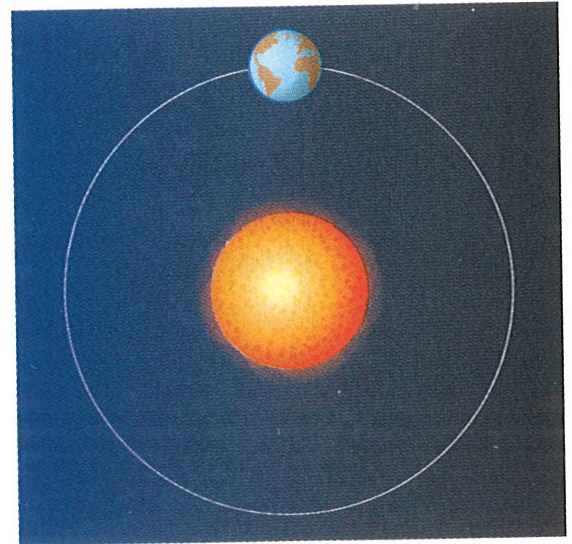
\includegraphics[scale=0.5]{terre}
\end{center}

\begin{questions}
	\question[2] Quelle est la distance parcourue par la Terre autour du Soleil pendant une année ?
	\fillwithdottedlines{3cm}
	
	\question[2] Calculer la vitesse de rotation de la Terre en km/h puis en km/s.
	\fillwithdottedlines{3cm}
\end{questions}


\section{Valeur, direction et sens (3 points)}

On a représenté ci-dessous, les vitesses de 4 objets (A, B, C et D) à un moment précis.

\begin{center}
	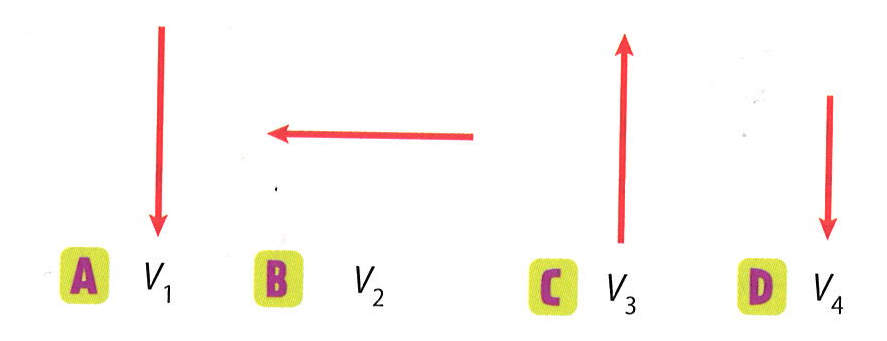
\includegraphics[scale=0.4]{exemples}
\end{center}

\begin{questions}
	\question \'A l'instant représenté, quels objets ont :
	\begin{parts}
		\part[1] la même direction ?
		%\fillwithdottedlines{1.5cm}
		
		\part[1] le même sens de déplacement ?
		%\fillwithdottedlines{1.5cm}
		
		\part[1] la même valeur ?
		%\fillwithdottedlines{1.5cm}
	\end{parts}

\end{questions}

\section{Représentation de la vitesse (6 points)}

\begin{questions}
	\question Représenter la vitesse d'un objet à un instant précis, dans les conditions suivantes  :
	
	\begin{parts}
		\part[2] \begin{itemize}
			\item Mouvement : horizontal de gauche à droite;
			\item Valeur de la vitesse : 25 m/s;
			\item \'Echelle choisie: 1 cm pour 10 m/s.
			
		\end{itemize}
	
		\makeemptybox{4cm}
		
		
		\part[2] \begin{itemize}
			\item Mouvement : chute verticale d'un objet;
			\item Valeur de la vitesse : 10 m/s;
			\item \'Echelle choisie: 1 cm pour 5 m/s.
			
		\end{itemize}
		
		\makeemptybox{4cm}
	\end{parts}

	\question[2] \'A l'aide d'un logiciel de traitement de vidéos, on peut repérer les positions successives prises par un point d'une grande roue lors de son mouvement.
	
	Sans tenir compte de la valeur de la vitesse, représenter la vitesse aux positions 3, 12, 22 et 33.
	
	\begin{center}
		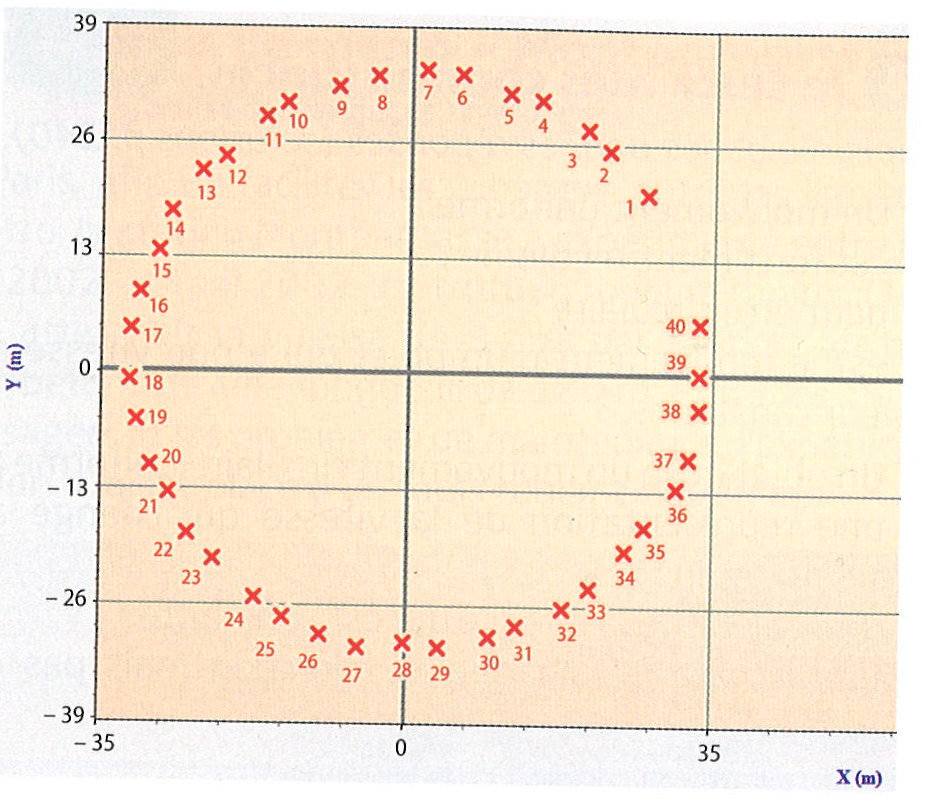
\includegraphics[scale=0.45]{roue}
	\end{center}
\end{questions}

\section{Proxima du centaure (4 points)}

Proxima du centaure est l'étoile la plus proche de notre système solaire. Sa lumière nous parvient après avoir parcouru \num{39700} milliards de kilomètres à la vitesse de \num{300000} km/s.

\begin{questions}
	\question[1] Quelle est la distance parcourue par la vitesse en un an ?
	\fillwithdottedlines{3cm}
	
	
	\question[1] Quelle est la durée, en année, du parcours de la lumière issue de cette étoile jusqu'à nous ?
	\fillwithdottedlines{4cm}
	
	\question[2] Quelle serait la durée, en année, de ce parcours pour une personne marchant à 5km/h ?
	\fillwithdottedlines{4cm}
\end{questions}
\section{Le lièvre et la tortue (7 points + 3 bonus)}

\begin{center}
	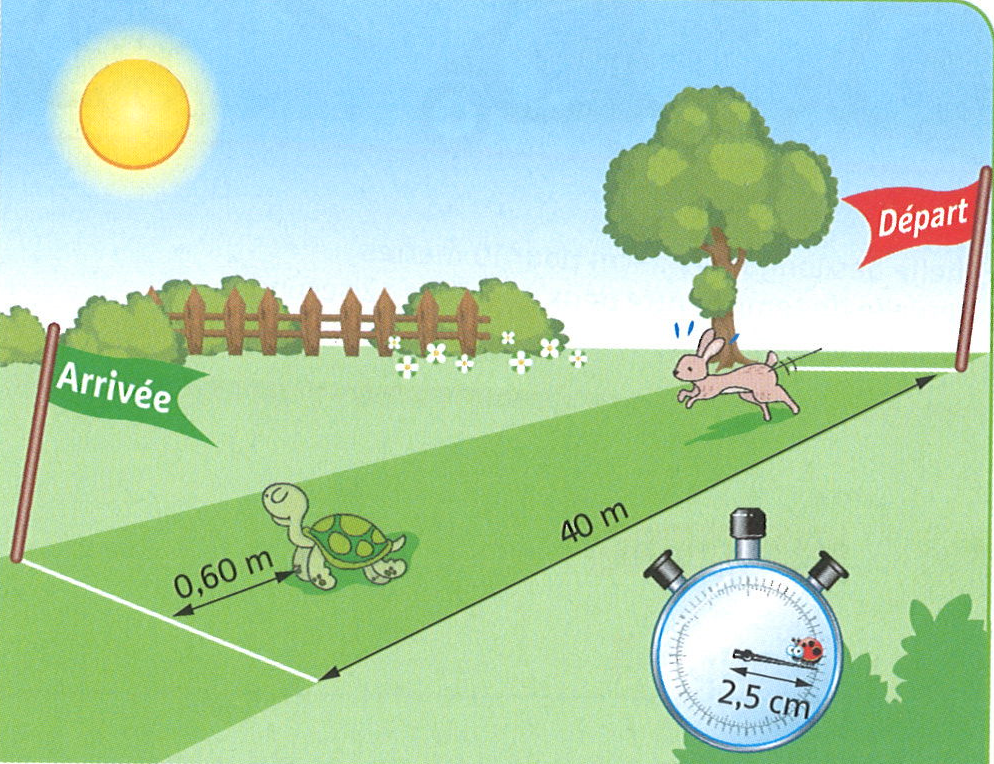
\includegraphics[scale=1.25]{lievre}
\end{center}

<<Rien ne sert de courir ; il faut partir à point>> est une maxime tirée de la fable <<le lièvre et la tortue>> de Jean de la Fontaine (1621 - 1695).\\


Après avoir fait la sieste sous un arbre à $\num{40.0}  m$  de la ligne d'arrivée, le lièvre se réveille et aperçoit la tortue qui le précède d'une distance $d = \num{39.4} m$. Elle file vers le succès dans cette ligne droite avec une vitesse de valeur constante $v_{tortue} = \num{0.2} m/s $.

Le lièvre se met alors à courir en accélérant jusqu'à atteindre une vitesse de valeur $v_{lievre} = \num{18.0} m/s$ et il s'y maintient.
\begin{questions}
	\question[1] Comment qualifie-t-on le mouvement de la tortue ?
	
%	\begin{parts}
%		\part[1] Comment qualifie-t-on le mouvement de la tortue ?
%		%\fillwithdottedlines{2cm}
%		%\part[1] Identifier et nommer les deux phases du  mouvement du lièvre.
%		%\fillwithdottedlines{2cm}
%		\part[2]Donner les trois caractéristiques de la vitesse de la tortue.
%		%\fillwithdottedlines{2cm}
%	\end{parts}

\vspace*{0.2cm}
	\question[2] Utiliser la formule de la vitesse
	
	\begin{parts}
		\part[1] Combien de temps faut-il à la tortue pour parcourir la distance qui la sépare de la ligne d'arrivée ?
		%\fillwithdottedlines{2cm}
		
		\part[1] Quelle distance peut parcourir le lièvre à sa vitesse maximale pendant cette même durée ?%maximale $d_{lievre}$ parcourrait le lièvre à sa vitesse maximale ?
		%\fillwithdottedlines{2cm}
	\end{parts}
\vspace*{0.2cm}
	\question[4] Lors de la phase d'accélération, on peut calculer la distance parcourue par le lièvre depuis l'arbre avec la formule suivante ($t$ est le temps que dure la phase d'accélération):
	
	\begin{equation*}
		distance = \num{4.5} \times t^2
	\end{equation*}

	\begin{parts}
		\part[2] On considère que cette accélération dure 2 secondes ; à quelle distance de l'arbre se trouve-t-il ?
		%\fillwithdottedlines{3cm}
		
		\part[1] A la fin de cette phase d'accélération, quelle distance lui reste-t-il à parcourir ?
		
		\part[1] Montrer alors qu'il a perdu la course.
		%\fillwithdottedlines{3cm}
	\end{parts}
\vspace*{0.2cm}

	\question[3] Une coccinelle, qui s'était endormie au bout de l'aiguille du chronomètre, fut entrainée dans son mouvement. \textbf{(Bonus)}
	
	\begin{parts}
		\part[1] Décrire la trajectoire de la coccinelle.
%		\fillwithdottedlines{2cm}
		
		\part[2] Calculer sa vitesse en cm/s, puis en m/s.
%		\fillwithdottedlines{3cm}
%		
%		\part[1] Tracer la flèche vitesse de la coccinelle en choisissant et précisant une échelle adaptée.
%		\makeemptybox{8cm}
%		
%		
%		
	\end{parts}
\end{questions}


%\section{Distance d'arrêt (8 points)}

Manon roule en scooter à 30 km/h. Elle est attentive. Soudain elle voit un enfant surgir imprudemment sur la route à 40 m d'elle.

\begin{multicols}{2}
	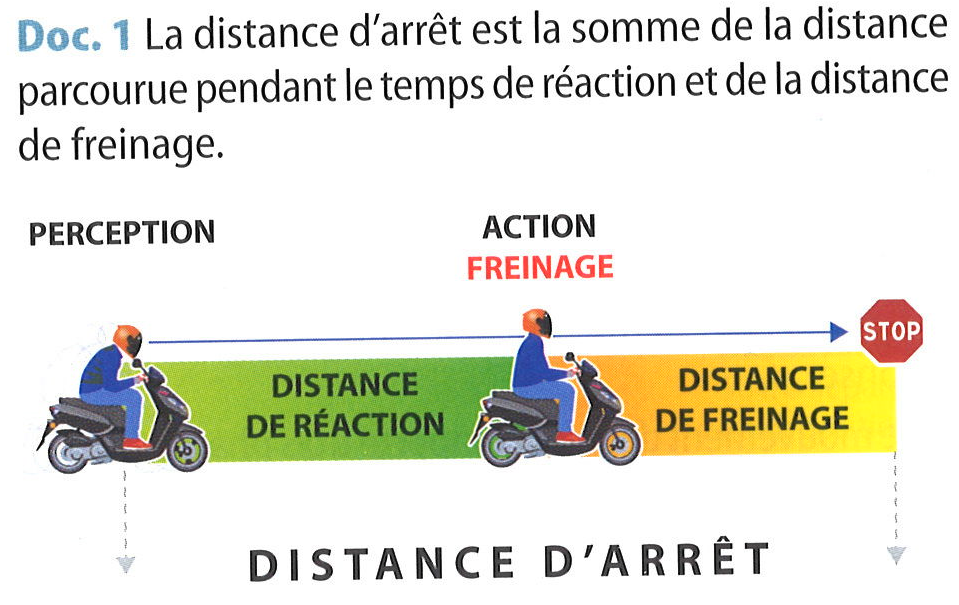
\includegraphics[scale=0.3]{dist_doc1}
	
	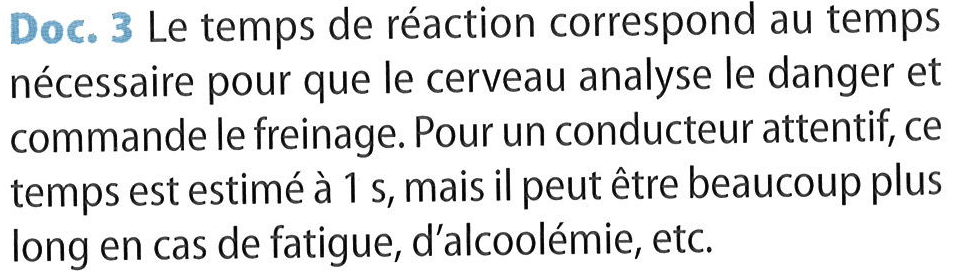
\includegraphics[scale=0.9]{dist_doc3}
	
	
	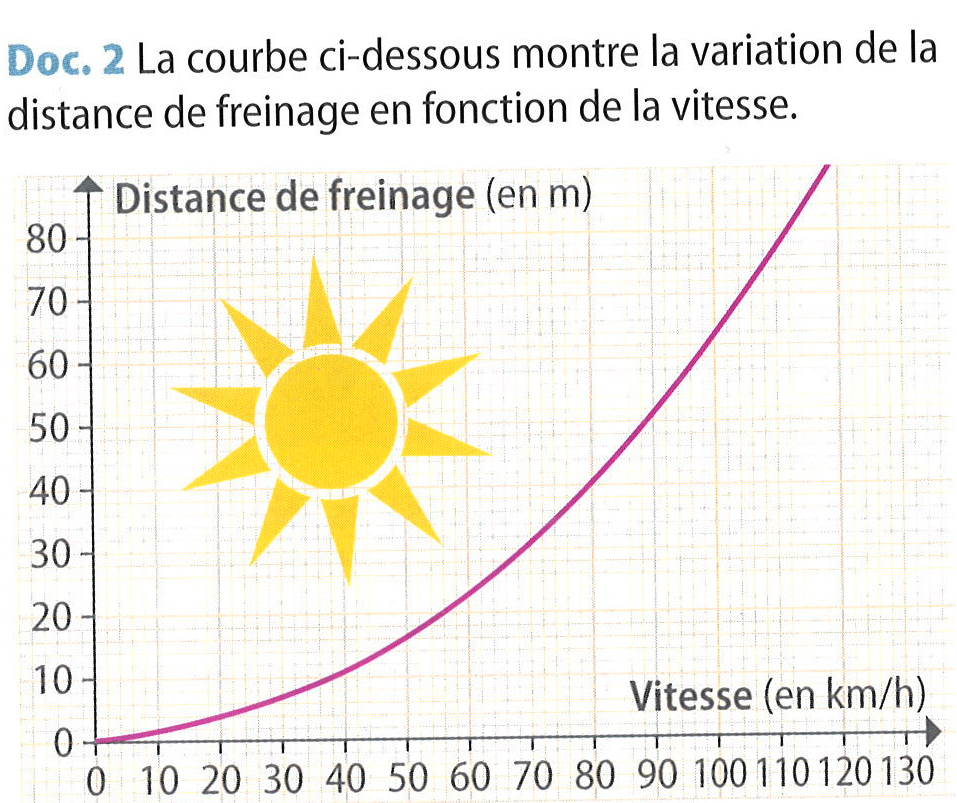
\includegraphics[scale=0.3]{dist_doc2}		
\end{multicols}

\begin{questions}
	\question[8] En utilisant les documents ci-dessus, expliquer, en détaillant le raisonnement si Manon peut éviter l'accident.  Détailler les calculs et comment les documents sont utilisés.
	
	\fillwithdottedlines{12cm}
\end{questions}






%\section{Profils de course (4 points)}

Après un cross de 4km, \'Ethan et Amine obtiennent le <<profil>> de leur course grâce à leur montre connectées : la distance parcourue s'affiche en fonction du temps.

\begin{center}
	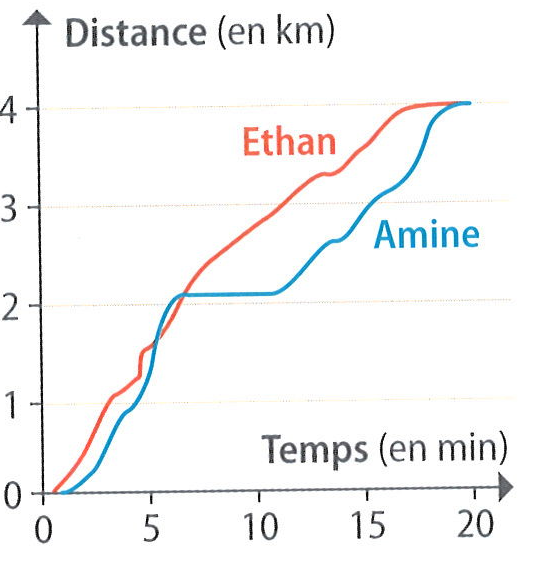
\includegraphics[scale=0.5]{cross}
\end{center}

\begin{questions}
	\question[1] \'Ethan et Amine ont-ils terminé la course ?
	\fillwithdottedlines{3cm}
	
	\question[1] Combien de temps ont-ils couru ?
	\fillwithdottedlines{3cm}
	
	\question[2] Lequel des deux s'est arrêté ? Expliquer la réponse.
	\fillwithdottedlines{4cm}
\end{questions}





\ \label{LastPage}

\end{document}